This work builds upon much prior research into powerful deep generative models,
self-supervised representation methods, and efficient transformer architectures.
We cover relevant work into deep generative models in \S\ref{subsec:agm} and
\S\ref{subsec:nagm}, vector-quantized image modelling in
\S\ref{subsec:vqmodelling}, a specific \acrshort{nar} generative model
\gls{sundae} in \S\ref{subsec:sundae}, and an efficient transformer architecture
in \S\ref{subsec:hourglass}. For a full review on generative modelling we direct
the reader to \citet{bondtaylor2021review}, and on \gls{sundae} and hourglass
transformers to \citet{savinov2022stepunrolled} and
\citet{nawrot2021hierarchical} respectively.

\begin{figure}[ht!]
    \centering
    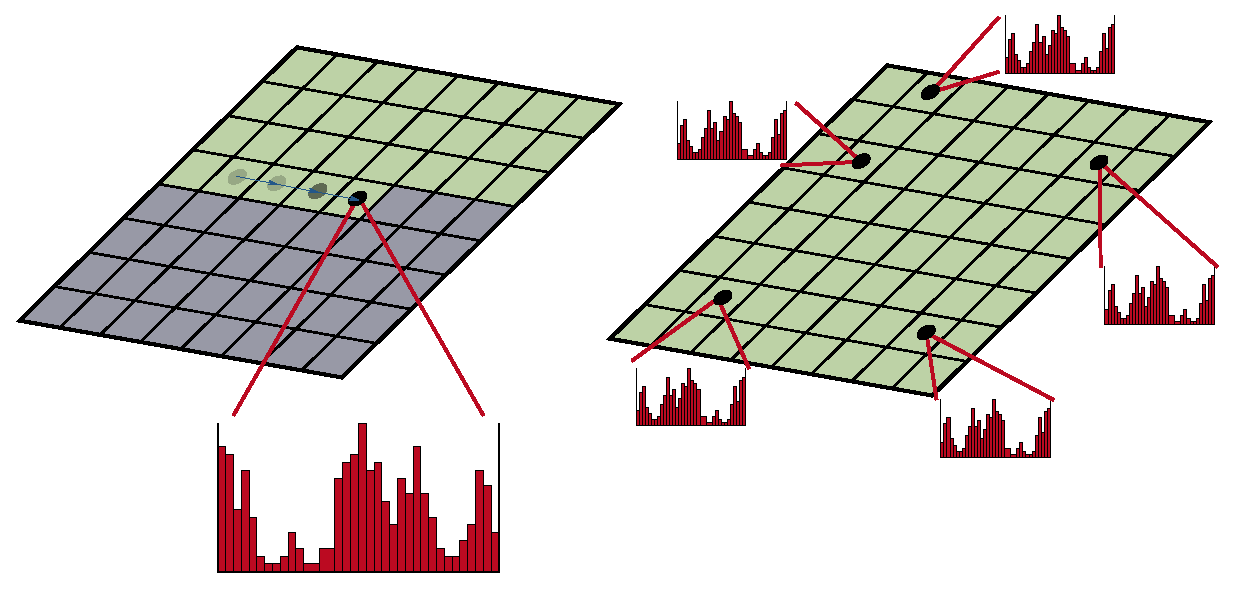
\includegraphics[width=\textwidth]{figures/AR-NAR.pdf}
    \caption{
        \textbf{Left:} Visualization of \acrfull{ar} sampling. \gls{ar} sampling
        proceeds one element at a time, meaning the number of sampling steps is
        equal to the dimensionality of the input. For each element, a
        probability distribution over possible discrete values is predicted and
        subsequently sampled from. Each prediction can only make use of past
        context -- indicated as a green position -- so not to violate the
        autoregressive property.
        \textbf{Right:} Visualization of \acrfull{nar} sampling. \Gls{nar}
        sampling samples an arbitrary number of elements in parallel, including
        elements previously sampled, allowing for self-correction. It freely
        uses all context available, allowing for flexible inpainting and
        better predictions.
    }
\end{figure}

\subsection{Autoregressive Generative Models}
\label{subsec:agm}

One major deep generative model family are \acrfull{ar} models, characterised by
a training and inference process based on the probabilistic chain rule. During
training, they learn to maximise the likelihood of the data they are trained on,
which leads to excellent mode coverage. Prior work using these methods resulted
in impressive results in terms of sample quality and diversity, but are
ultimately impractical in most real world applications due to their slow
sampling speed.

The slow speed is due to their sequential nature, defined by the chain
rule of probability. Given an input $\image = \{ \pixel{1}, \pixel{2}, \dots,
\pixel{n} \}$, an \gls{ar} model $p_\theta(\cdot)$ generates new
samples sequentially:
\begin{equation}\label{eq:ar}
    p_\theta(\image) = p_\theta(\pixel{1}, \dots, \pixel{n}) =
    \prod\limits^{n}_{i=1} p_\theta(\pixel{i} \vert \pixel{1}, \dots, \pixel{i-1})
\end{equation}
meaning that the number of sampling steps is equal to the size of the
decomposition of $\image$, giving an iteration complexity of $\bigO{n}$.

For certain tasks, the ordering of the decomposition of $\image$ is obvious, for
example on text or speech. For images this is less clear, but typically a raster
scan ordering is used~\cite{parmar2018image}. Certain \gls{ar} models are
order-agnostic~\cite{hoogeboom2021autoregressive}, allowing for arbitrary
ordering to be used during training and inference.

One class of \gls{ar} models are \glspl{rnn} which are an early example of using
neural networks to model sequential data such as text, audio, time-series data,
or even handwriting strokes. Though they can be used as classification or
regression models, they are also suited for use as generative models by
modelling the relationship in Equation~\ref{eq:ar}. They suffer from a number of
issues, most infamously vanishing gradients~\cite{pascanu2012rnn} and inability
to model long-range relationships between elements in the input.
\Glspl{lstm}~\cite{hoch1997lstm} improved upon \glspl{rnn} by introducing
dedicated memory units, allowing for the modelling of long-range
relationships. \Glspl{gru}~\cite{cho2014gru} simplified the \gls{lstm}
architecture whilst retaining good performance. With the advent of transformer
architectures~\cite{vaswani2017attention}, modelling longer relationships became
possible, even at a full-document level. It also introduced the capability to
train on all sequence elements in parallel through the use of causal masking,
therefore not violating the autoregressive property. Inference must still be
done in a sequential manner, however.

Applying \gls{ar} models to images followed a similar progression.
PixelRNN~\cite{oord2016pixelrnn} used two-dimensional recurrent layers and
residual connections to model the distribution of raw pixel values. The same
paper also introduced PixelCNN, which had worse performance but is faster to
train. These were extended to allow for conditional generation
in~\cite{oord2016pixelcnn}. Later work augmented PixelCNN with self-attention
mechanism, forming PixelSnail~\cite{chen2017snail}, which can model longer
relationships than a fully convolutional or recurrent architecture. Image
Transformer~\cite{parmar2018image} later applied transformer architectures to
the same task through an effective but conceptually simple approach. In all
cases, the iteration complexity is still $\bigO{n}$, a property intrinsic to
\gls{ar} models.

\subsection{Non-autoregressive Generative Models}
\label{subsec:nagm}

\Acrfull{nar} generative models include \glspl{gan}, \glspl{sbm} and
\glspl{ddpm}, and flow-based models. The number of sampling steps in \gls{nar}
models is independent of the data dimensionality, however the actual number of
steps varies greatly: from single-step generation in \glspl{gan} to many
thousands in early diffusion models.

The most infamous class of \gls{nar} generative model -- or generative model
altogether -- are \acrfullpl{gan}~\cite{goodfellow2014gan}. \Glspl{gan} consist
of two components: a generator that creates samples from latent variables, and a
discriminator that attempts to distinguish samples from the dataset from samples
from the generator~\cite{goodfellow2014gan}. They are known for high-fidelity
samples, fast sampling, unstable training, and tendency to collapse onto a
subset of modes of the data distribution, due to not optimising directly for
likelihood. This is reflected in its relatively low-diversity samples.
Nonetheless, the quality and speed of the samples have made them a popular
choice in a variety of applications, including unconditional and conditional
generation~\cite{tero2018stylegan,andrew2018biggan}, image and audio
synthesis~\cite{liu2020audiogan}, and style transfer~\cite{zhu2017cyclegan}.
They can be applied to discrete data~\cite{autume2019scratchgan}, but are
less effective due to the non-differentiability of discrete samples.

\Acrfullpl{vae}~\cite{kingma2013vae} are a class of generative model which
permit sampling in a single forward pass like \glspl{gan}, but are trained to
maximise likelihood. Specifically, \glspl{vae} map inputs to latent variables
that follow some easy to sample, but sufficiently complex, prior distribution. A
common choice is a multivariate Gaussian with diagonal
covariance~\cite{kingma2013vae}. A decoder network maps latent codes to the data
distribution. Although this approach is successful on simple datasets, on
complex datasets the samples and reconstructions become blurry, suggesting a
simple prior is insufficient to model the data distribution. Later work extended
\glspl{vae} to be hierarchical, having multiple Gaussian
priors~\cite{arash2020nvae,child2020vqvae}, which was found to outperform
\gls{ar} models.

Another non-adversarial \gls{nar} class that permits sampling in a single
forward pass are normalizing flows, a class of generative model that allows for
exact likelihood calculation~\cite{dinh2014nice,dinh2016density,kingma2018glow}.
They consist of many invertible layers that transform samples from a known prior
distribution into samples from the data distribution. Each transformation must
satisfy two properties: being invertible and having an easy to compute Jacobian
for scaling~\cite{dinh2014nice,dinh2016density}. This means the architectural
choices are restricted, making them parameter inefficient. They also must
operate at the same dimensionality for each layer, making the training of deep
networks difficult.

\Acrfullpl{ddpm}~\cite{ho2020ddpm,dhariwal2021ddpm} and
\acrfullpl{sbm}~\cite{song2019sbm,song2020sde,song2021mlt,vahdat2021sbmlatent}
have garnered much interest in recent work, with the former learning to estimate
the noise and the latter trained to remove noise, given samples from a
corrupting forward process. Either method can then be used to move from 
noise to data, forming a generative model~\cite{song2019sbm}. Both are slow to
sample from, but produce high quality samples that rival those of
\glspl{gan}~\cite{dhariwal2021ddpm} whilst not suffering from mode collapse. The
slow sampling speed can be remedied using a variety of techniques, such as
operating over a smaller latent space~\cite{vahdat2021sbmlatent}, devising
efficient SDE solvers~\cite{martineau2021fast}, or by diffusing ``velocities'',
thus simplifying the denoising task~\cite{dockhorn2021langevin}. Unlike
\glspl{gan}, both models can operate on discrete data, either by projecting
discrete data into a continuous latent space~\cite{vahdat2021sbmlatent} or with
a discrete diffusion framework~\cite{austin2021structured}, the latter of which
bridges the gap between diffusion, autoregressive, and mask-based representation
models such as BERT~\cite{devlin2019bert}. Despite the iteration complexity no
longer being $\bigO{n}$, there is a still a gap between the sampling speed of
adversarial and non-adversarial methods.

\subsection{Vector Quantized Image Modelling}
\label{subsec:vqmodelling}

Learning useful latent representations, also known as latent codes, in an
unsupervised manner is a key challenge in machine learning. Historically, these
representations have been continuous, but in recent work they are often
discrete. An early example is \gls{vqvae}~\cite{oord2017vqvae}, which has three
main components: an encoder network, a codebook, and a decoder. The encoder
network outputs a compressed continuous representation of the input, and the
codebook $\vqganCodebook$ quantizes these representations, outputting discrete
indices from $1$ to the codebook size $\vqganNbLatents$. Each index $i$ maps to
one of the codebook embeddings (codewords) $e_i$. The decoder maps the quantized
embeddings to a lossy reconstruction of the input. \Gls{vqvae} is trained
end-to-end to reconstruct the input and to minimize the codebook
loss~\cite{oord2017vqvae}. Once trained, an auxiliary generative model is
trained to generate the discrete latent representations. The decoder then
decodes the sampled latent, producing the final sample. In the original work,
PixelCNN was used to generate the discrete latent codes~\cite{oord2017vqvae},
though any generative model for discrete data can be used.

\begin{figure}[ht!]
    \centering
    \includegraphics[width=\textwidth]{figures/vq.pdf}
    \caption{
        Visualisation of a vector-quantization image model. An encoder model
        extracts continuous representations from the input. Vector
        quantization is then used to map each continuous embedding to the
        closest entry in the codebook. A decoder model takes the discretized
        embeddings outputs a lossy reconstruction of the input. We 
        generate a dataset of latent representations from an image dataset 
        by iterating $\image \in \imageDataset$ and appending the resulting
        discrete representation $\latent$ to a set $\latentDataset$.
    }
    \label{fig:vq}
\end{figure}

Later approaches extended \gls{vqvae} to multiple hierarchical codebooks in
\acrshort{vqvae}-2~\cite{razavi2019generating}. Though it can be extended to any
number of codebooks, they experimented with at most three, applying it to $1024
\times 1024$ images. They then sampled the hierarchical discrete representations
using multiple PixelSnail~\cite{chen2017snail} models, each code conditioned on
all previous levels in the hierarchy. Though faster to sample than generating
pixels directly, at such a resolution and with multiple representation levels,
sampling times were still very slow.

Aside from sampling autoregressively, a reason for the slow sampling speed is
the large spatial resolution of the discrete codes. Albeit smaller than the
original input, \gls{vqvae} is limited in how much it can compress the signal
via a simple reconstruction objective before it loses significant perceptual
quality, due to the rate-distortion trade-off. For example, the original
\gls{vqvae} only has a downsampling rate of
$\vqganDownsample=4$~\cite{oord2017vqvae} and \gls{vqvae}-2 has a top-level rate
of $\vqganDownsample=32$ but requires three discrete latent codes to achieve
this~\cite{razavi2019generating}. By introducing perceptual and adversarial loss
terms, \gls{vqgan}~\cite{esser2021taming} is able to achieve a compression rate
of $\vqganDownsample=32$ with only a single discrete latent representation
whilst maintaining high quality reconstructions~\cite{esser2021taming}. However,
the greater weighting on perceptual and adversarial loss does mean that
\gls{vqgan} sometimes edits the reconstructions, rather than faithfully
reconstruct the input. Later, improvements including differential data
augmentation~\cite{bondtaylor2021unleashing}, codebook improvements, and a
transformer-based architecture~\cite{yu2021vqgan} improved reconstruction
quality further, but still rely on adversarial components.

Designed for audio compression~\cite{zeghidour2021soundstream},
residual \gls{vq} proposes the use of multiple codebooks to recursively quantize
and refine the residual of the input. This produces multiple discrete
representations, which can later be reconstructed by the decoder to recover
the waveform. Individual codebooks can be dropped out, allowing
for variable bit-rates~\cite{zeghidour2021soundstream}. Concurrently to our
work, \citet{lee2022rqvae} used residual \gls{vq} to represent images with 
$\vqganDownsample=32$ and then trained a spatial transformer 
to autoregressively predict the stack of discrete tokens at a given spatial
location, allowing for fast sampling even with multiple levels of discrete
representations~\cite{lee2022rqvae}. A summary of each \gls{vq} model and
their latent and codebook sizes is shown in Table~\ref{tab:vq}.

\begin{table}[ht]
    \centering
    \begin{tabular}{|c|c|c|c|c|c|}
        \hline
        \textbf{Model} & \textbf{Input Size} & \textbf{Latent Shape} & \textbf{Codebook Size} & \textbf{FID/val} & \textbf{FID/train} \\
        \hline
        VQ-VAE & $128 \times 128$ & $32 \times 32$ & $512$ & -- & -- \\
        \hline
        VQ-VAE-2 & $256 \times 256$ & $64 \times 64$ \& $32 \times 32$ & $512$ & --& $\sim 10$ \\
                 & $1024 \times 1024$ & $128 \times 128$ \& $64 \times 64$ \& $32 \times 32$ & $512$ & -- & -- \\
        \hline
        DALLE & $256 \times 256$ & $32 \times 32$ & $8192$ & $32.01$ & $33.88$ \\
        \hline
        VQ-GAN & $256 \times 256$ & $16 \times 16$ & $1024$ & $7.94$ & $10.54$ \\
        & $256 \times 256$ & $16 \times 16$ & $16384$ & $4.98$ & $7.41$ \\
        & $256 \times 256$ & $32 \times 32$ & $8192$ & $1.49$ & $3.24$ \\
        & $256 \times 256$ & $64 \times 64$ \& $32 \times 32$ & $8192$ & $1.45$ & $2.78$ \\
        \hline
        RVQ-VAE & $256 \times 256$ & $8 \times 8 \times 2$ & $16384$ & -- & $10.77$ \\
        & $256 \times 256$ & $8 \times 8 \times 4$ & $16384$ & -- & $3.20$ \\
        & $256 \times 256$ & $8 \times 8 \times 8$ & $16384$ & -- & $2.69$ \\
        & $256 \times 256$ & $8 \times 8 \times 16$ & $16384$ & -- & $1.83$ \\
        \hline
    \end{tabular}
    \caption[Table]{Summary of various \acrfull{vq} methods. The trend with
    \gls{vq} image models is increasing compression rates $\vqganDownsample$ and
    codebook sizes. However, to achieve these compression rates techniques such
    as perceptual and adversarial losses must be used.}
    \label{tab:vq}
\end{table}

A typical strategy for selecting which codebook vector $e_i$ to map to a given
embedding is to compute the Euclidean distance between the embedding and each
codeword centroid, and then pick the $\arg\min$~\cite{oord2017vqvae}, known as a
$k$-means strategy. This can result in ``codebook collapse'', where certain
codewords never get used, limiting the effective capacity of the model. An
alternative is to use Gumbel-Softmax~\cite{jang2016gumbel} to select codewords,
which increases codebook utilisation but leads to worse reconstruction
quality~\cite{bondtaylor2021unleashing}.
The issue of codebook collapse is significant and there have been a number
of attempts to address it. \cite{yu2021vqgan} found that a lower codeword
dimension and codeword normalization improved utilisation.
\cite{zeghidour2021soundstream} proposed setting a threshold for ``stale'' codes,
and reinitialising them to a random vector from the current batch when they
fall below this threshold. \cite{lee2022rqvae} proposed the sharing of a single
codebook across many quantizers and stochastically sampling the
codes as a function of their distance to each codeword centroid, rather than
deterministically using the $\arg\min$.

All previously described approaches use \gls{vq} models to enhance existing
\gls{ar} models, primarily to improve sampling speeds by reducing the spatial
dimension they operate over. Little work directly addresses the discrete prior
model. Discrete diffusion models~\cite{austin2021structured} are a \gls{nar}
approach to generating discrete data, applied to \gls{vqgan} latents in
\citet{bondtaylor2021unleashing}, resulting in fast sampling, flexible
inpainting, and high fidelity outputs.

\subsection{Step-unrolled Denoising Autoencoder}
\label{subsec:sundae}

\Gls{sundae}~\cite{savinov2022stepunrolled} is a \gls{nar} text generative model
evaluated on three language modelling tasks: unconditional text-generation,
inpainting of Python code, and machine translation -- setting a new
state-of-the-art among \gls{nar} models for the
latter~\cite{savinov2022stepunrolled}. It is capable of fast sampling, producing
high quality samples in as few as 10 steps.

It is trained using a denoising objective, akin to 
BERT's objective~\cite{wang2019bert} but with multiple denoising steps.
Given a uniform prior $p_0$ over some space $\latentSpace = \{1, \dots,
\vqganNbLatents\}^N$ where $N$ is the size of the space and $v$ is the
vocabulary size, consider the Markov process $\latent_t \sim \sundae(\cdot \vert
\latent_{t-1})$ where $\sundae$ is a neural network parameterised by
$\sundaeParameters$, then $\{\latent_t\}_t$ forms a Markov chain. This gives a
$t$-step transition function: 
\begin{equation}\label{eq:markov} p_t(\latent_t
    \vert \latent_0) = \sum\limits_{\latent_1, \dots, \latent_{t-1} \in
    \latentSpace} \prod\limits^t_{s=1} \sundae(\latent_s | \latent_{s-1})
\end{equation}
\cite{savinov2022stepunrolled} and, given a constant number of steps
$\markovSteps$, our model distribution $p_\markovSteps(\latent_\markovSteps
\vert \latent_0)p_0(\latent_0)$ -- which is clearly intractable.

Instead, \gls{sundae} uses an \textit{unrolled denoising} training method that
uses a far lower $\markovSteps$ than is used for
sampling~\cite{savinov2022stepunrolled}. To compensate, they unroll the Markov
chain to start from corrupted data produced by a \textit{corruption
distribution} $\latent_0 \sim \corruptionDistribution(\cdot \vert \latent)$
rather than from the prior $p_0$ so the model during training sees inputs alike
those seen during the full unroll at sample time~\cite{savinov2022stepunrolled}.
Typically, $\markovSteps = 2$ is used during training, as a single step would be
similar to BERT's objective~\cite{devlin2019bert} which would not be performant
as seen in earlier work using BERT as a random field language
model~\cite{wang2019bert}.

The training objective of \gls{sundae} is the average of all
cross-entropy losses on the chain after $t$ steps, which is shown to form an
upper bound on the actual negative
log-likelihood~\cite{savinov2022stepunrolled}. Increasing $\markovSteps$
leads to a minor improvement in performance, but considerably slows down
training~\cite{savinov2022stepunrolled} and increases memory usage.

One advantage of this approach is that sampling starts from random tokens,
rather than a ``masking''
token~\cite{bondtaylor2021unleashing,austin2021structured}. Unmasking approaches
means that $\markovSteps \leq N$ as at minimum, one token is unmasked per step.
Additionally, it allows the model to ``change its mind'' about previously
predicted elements during sampling, permitting fine-grained adjustments and
correction of errors.

\subsection{Hourglass Transformers}
\label{subsec:hourglass}

Vanilla transformers incur a memory complexity of $\bigO{L^2}$ for each
block~\cite{vaswani2017attention}, dominated by costly multi-head self-attention
mechanisms. Most research into efficient transformers focuses on improving the
efficiency of the attention mechanisms using sparse attention
patterns~\cite{child2019generating} or through linear complexity
approximations~\cite{xiong2021nystromformer}.

Recent work has focused on making the architecture itself more efficient. Funnel
transformers~\cite{dai2020funneltransformer} progressively downsamples the input
sequence and hence reduces the computational cost of the model. The saved
\glspl{flop} can then be reassigned to create deeper or wider models and thus
outperform vanilla transformers given the same computational
budget~\cite{dai2020funneltransformer}. However, the final layer does not
operate at the same granularity as the input, making it unusable for tasks such
as per-token classification or generative modelling. Hourglass
transformers~\cite{nawrot2021hierarchical} include both up- and down-sampling
mechanisms, resulting in a computational saving whilst being general-purpose
models.

\subsection{Summary of Trends in Deep Generative Modelling}
\label{subsec:trends}

Deep generative modelling research is a fast moving, complex and turbulent field
to follow. Nonetheless, it is worthwhile to distill advancements into a
selection of high level trends.

\textbf{Improving quality and efficiency in non-adversarial generative models} -- 
\Glspl{gan} have long dominated as the pinnacle of sample quality and
efficiency. Despite this, they are plagued by previously discussed issues,
motivating research into non-adversarial approaches of equal quality to
\glspl{gan}. Certain non-adversarial solutions do beat \glspl{gan} in quality,
but \glspl{gan} still dominate in terms of sample speed, making them the
standard in real-world generative modelling applications -- bar cutting
edge applications~\cite{ramesh2021dalle,ramesh2022dalle2}. Hence the trend is
the simultaneous improvement in efficiency and quality, as it is clear that
without both, adoption in practise will not occur. Satisfying these speed and
quality requirements with a non-adversarial solution would in turn satisfy the
aforementioned generative modelling trilemma~\cite{xiao2021trilemma}.

\textbf{Autoregressive to non-autoregressive models} -- 
\Gls{nar} models offer a number of advantages over \gls{ar} models as discussed
in earlier sections. It is clear that \gls{nar} solutions will soon be a default
over \gls{ar} methods, seen by observing that initial proposed methods and
subsequent improvements often replace \gls{ar} components with \gls{nar}
components. For example: sampling \gls{vqgan} latents with \gls{ar}
transformers~\cite{esser2021taming} to using discrete diffusion
models~\cite{bondtaylor2021unleashing}; DALL·E using \gls{ar}
sampling~\cite{ramesh2021dalle} to DALL·E 2 using diffusion
models~\cite{ramesh2022dalle2}.

\textbf{Class conditional to zero-shot conditional generative models} -- One
especially popular trend is the shift from specifying a set of predefined
classes when conditioning a model, to full zero-shot generation. This is usually
realised by jointly learning text and image embeddings, then encoding a text
prompt at sample time to condition the
model~\cite{ramesh2021dalle,ramesh2022dalle2,rombach2021highresolution,lee2022rqvae}.
This allows for a much higher degree of creative control -- an all too often
overlooked property -- and can be easily integrated with existing architectures.
However, they require large amounts of labelled images and associated text
prompts, usually scraped from the
internet~\cite{rombach2021highresolution,ramesh2021dalle,ramesh2022dalle2}. This
makes bias and dangerous content introduced by the training data much harder to
control and filter, influencing the resulting samples~\cite{mishkin2022risks}.
Nonetheless, it is clear that the natural language conditioning of generative
models will persist.

\textbf{Use of a vector-quantized discrete prior} -- 
Though \gls{vq} models have helped produce excellent results both within
generative
modelling~\cite{razavi2019generating,esser2021taming,bondtaylor2021unleashing,rombach2021highresolution,ramesh2021dalle,yu2021vqgan,lee2022rqvae}
and elsewhere~\cite{zeghidour2021soundstream}, excellent results can also be
obtained without the use of
them~\cite{child2020vqvae,arash2020nvae,hazami2022efficient}, especially with
diffusion
models~\cite{song2019sbm,song2020sde,dhariwal2021ddpm,song2021mlt,xiao2021trilemma,vahdat2021sbmlatent,martineau2021fast,dockhorn2021langevin}.
The advantage of using a \gls{vq}-based approach is the
reduction of the spatial resolution that the generator model must operate
over, aiding in scaling to higher resolutions and improving sampling speeds.
However, the two-stage training approach can be unwieldy without pretrained
\gls{vq} models and makes inpainting more involved. Additionally,
they are plagued with issues such as codebook
collapse~\cite{esser2021taming,bondtaylor2021unleashing,yu2021vqgan}, limiting
the potential capacity of the model. It remains to be seen whether \gls{vq}
models will continue being a popular component in generative modelling pipelines,
or be rendered obsolete.

